\documentclass[20pt]{beamer}
\usepackage[]{bookmark}
\usepackage[utf8]{inputenc}
\usepackage{amsmath}
\usepackage{amsfonts}
\usepackage{amssymb}
\usepackage{tikz}
\usepackage{xcolor}
\usepackage[dutch]{babel}
\usepackage{sansmathaccent}
\usepackage{graphicx}
\usepackage{pgfplots}

\usepackage[style=authoryear,backend=biber]{biblatex}

\addbibresource{bibliography2.bib} 
\pdfmapfile{+sansmathaccent.map}

\title{RMC voor lineaire ODEs}
\author{Isidoor Pinillo Esquivel }
\usetheme{Madrid}
\date{}

\begin{document}

% 1 min
\begin{frame}
    \titlepage
\end{frame}
% 2 min
\begin{frame}
    \frametitle{Grid-Free Monte Carlo}
    \cite{sawhney_grid-free_2022}
    \begin{figure}[h!]
        \centering
        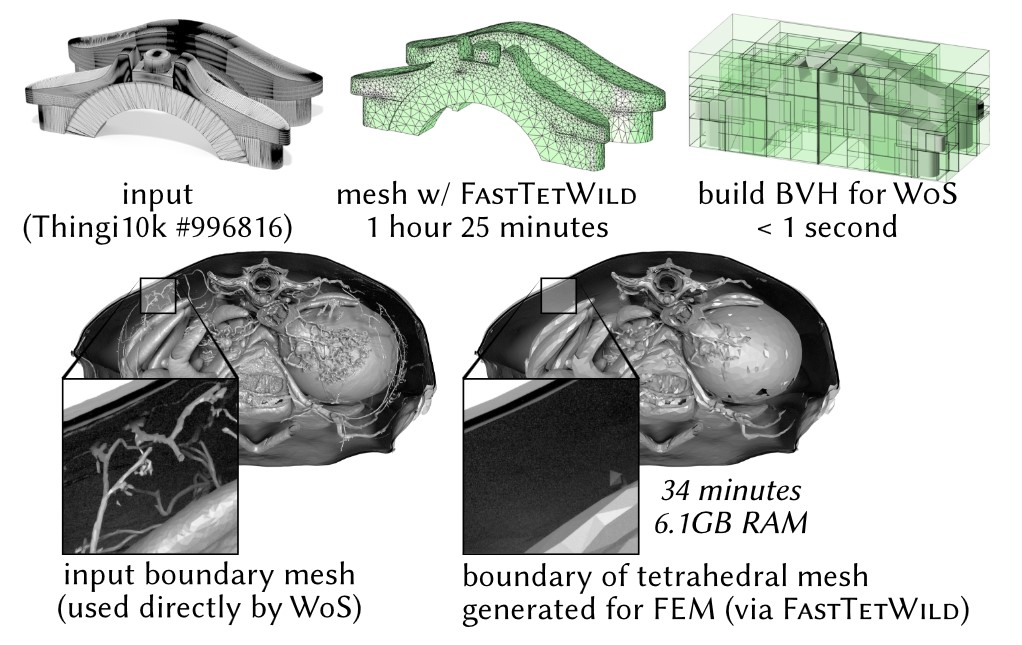
\includegraphics[width=0.8\textwidth]{imgs/Grid_free_comparison.jpg}
        \label{fig:grid_free_comparison}
    \end{figure}
\end{frame}

% 2 min
\begin{frame}
    \frametitle{Monte Carlo}
    \vspace{-1cm}
    \begin{align}
        \int_{0}^{1} f(s) ds & = E[f(U)]                                   \\
                             & \approx \frac{1}{n} \sum_{j=1}^{n} f(U_{j}) \\
        \text{met } U_{j}    & \sim \text{Uniform}(0,1)
    \end{align}
\end{frame}

\begin{frame}
    \frametitle{Monte Carlo Fout Analyse}
    \vspace{-1cm}
    \begin{equation}
        \text{fout} = O_{p} \left(\sqrt{\frac{\text{Var}(f(U))}{n}} \right) \text{(CLT)}
    \end{equation}
    \pause
    \vspace{-1cm}
    \begin{align}
         & \sqrt{\text{Var}  (f(U))}      \\
         & = \sqrt{E[(f(U)-E[f(U)])^{2}]} \\
         & = ||f-E[f(U)]||_{2}            \\
         & \sim ||f||_{2}
    \end{align}
\end{frame}

\begin{frame}
    \frametitle{Waarom Monte Carlo?}
    \begin{itemize}
        \item paralleliseerbaar
        \item dimensie onafhankelijke convergentie
        \item complexe geometrie
    \end{itemize}
\end{frame}

\begin{frame}
    \frametitle{Waarom ODEs?}
    \begin{itemize}
        \item grid-free + tijdafhankelijkheid?
        \item ODEs simpeler als PDEs
    \end{itemize}
\end{frame}

\begin{frame}
    \frametitle{Stochastic Gradient Descent}
    \vspace*{-0.3cm}
    \begin{center}
        SGD = GD + unbiased gradients
    \end{center}
    \vspace*{-0.3cm}
    \pause
    \begin{align}
        \action<+->{f(x)        & = \frac{1}{n}\sum_{j=1}^{n} f_{j}(x)  }        \\
        \action<+->{\nabla f(x) & = \frac{1}{n}\sum_{j=1}^{n} \nabla f_{j}(x)  } \\
        \action<+->{            & =  E[\nabla f_{J}(x)]}
    \end{align}
\end{frame}

\begin{frame}
    \frametitle{Russische Roulette Voorbeeld}
    \vspace*{-1cm}
    \begin{align}
        \action<+->{Z         & = U + \frac{f(U)}{1000}  }                          \\
        \action<.->{U         & \sim \text{Uniform}(0,1), \text{ } f \text{ duur} } \\
        \action<+->{\tilde{Z} & = U + B \left(\frac{1}{100}\right)\frac{f(U)}{10}}  \\
        \action<.->{B(p)      & \sim \text{Bernoulli}(p)}
    \end{align}
\end{frame}

% 2 min
\begin{frame}
    \frametitle{Control Variates}

    \begin{columns}[t]
        \begin{column}{0.55\textwidth}
            \vspace*{-2cm}
            \begin{figure}[h]
                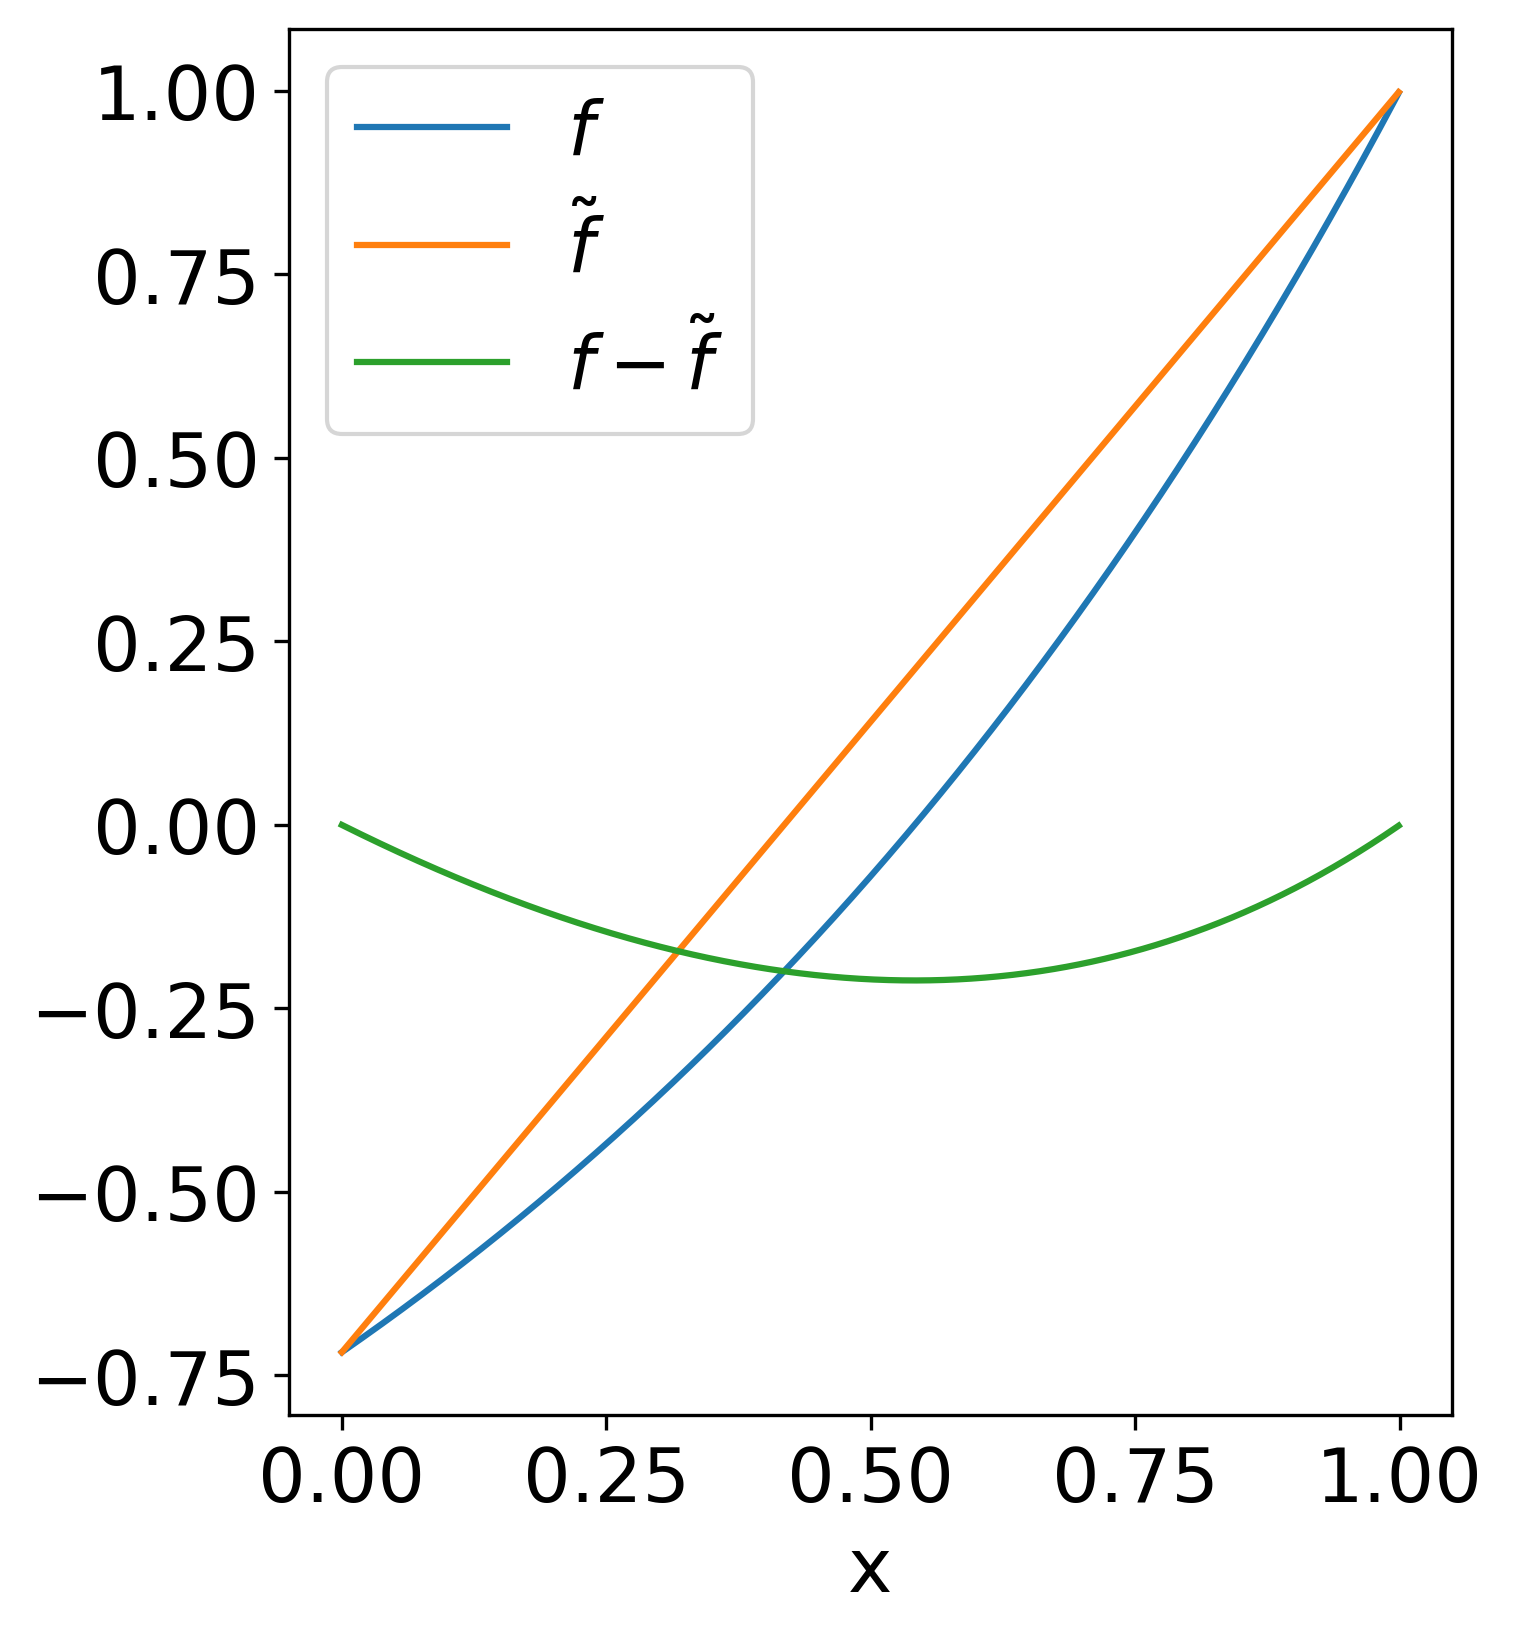
\includegraphics[height=0.8\textheight]{"imgs/control_variate.png"}
            \end{figure}
        \end{column}
        \begin{column}{0.45\textwidth}
            \pause
            \[
                f  \approx \tilde{f} \rightarrow
            \]\pause
            \vspace*{-1cm}
            \[
                ||f-\tilde{f}||_{2} \le ||f||_{2}
            \]
            \pause
            \vspace*{-1cm}
            \begin{center}
                weet $\int \tilde{f}(s)ds$ \\
                bv $\tilde{f}$ lineair
            \end{center}

        \end{column}
    \end{columns}

\end{frame}

% % 2 min
% \begin{frame}
%     \frametitle{RMSE vs fout begrenzing}
%     \begin{itemize}
%         \item verschil (+ formule)
%         \item mss: steins paradox (yt video)
%         \item MSE decompositie
%         \item tabel: $0$ variantie vs $0$ bias
%     \end{itemize}
% \end{frame}

% 2 min
\begin{frame}
    \frametitle{Trapezium Monte Carlo}
    \fontsize{15}{17}\selectfont
    \begin{center}
        Trap MC = \textcolor{red!90!black}{Russische Roulette} + Control Variates
    \end{center}
    \pause
    \vspace{-0.2cm}
    \begin{align}
        \action<+->{ & \textcolor{blue!95!black}{\int_{x}^{x+\Delta x} f(s) ds}     }          \\
        \action<+->{ & = \textcolor{orange!95!black}{\int_{x}^{x+\Delta x}  \tilde{f}(s) ds} +
        \textcolor{green!80!black}{\int_{x}^{x+\Delta x}  f(s) - \tilde{f}(s) ds}  }           \\
        \action<+->{ & =\textcolor{orange!95!black}{\Delta x \frac{f(x) + f(x+\Delta x)}{2}}
            + E \left[\textcolor{red!90!black}{l B\left( \frac{1}{l}\right)}
        \textcolor{green!80!black}{(f(S_x) - \tilde{f}(S_x))}\right]}                          \\
        \action<+->{ & \text{waar }
            \textcolor{red!90!black}{\text{ l}} = \text{ RR rate},
            \textcolor{green!80!black}{S_x} \sim \text{Uniform}(x,x+\Delta x)
        }
    \end{align}
\end{frame}

\begin{frame}
    \frametitle{Trapezium Monte Carlo}
    \begin{columns}[t]
        \begin{column}{0.55\textwidth}
            \vspace*{-2cm}
            \begin{figure}[h]
                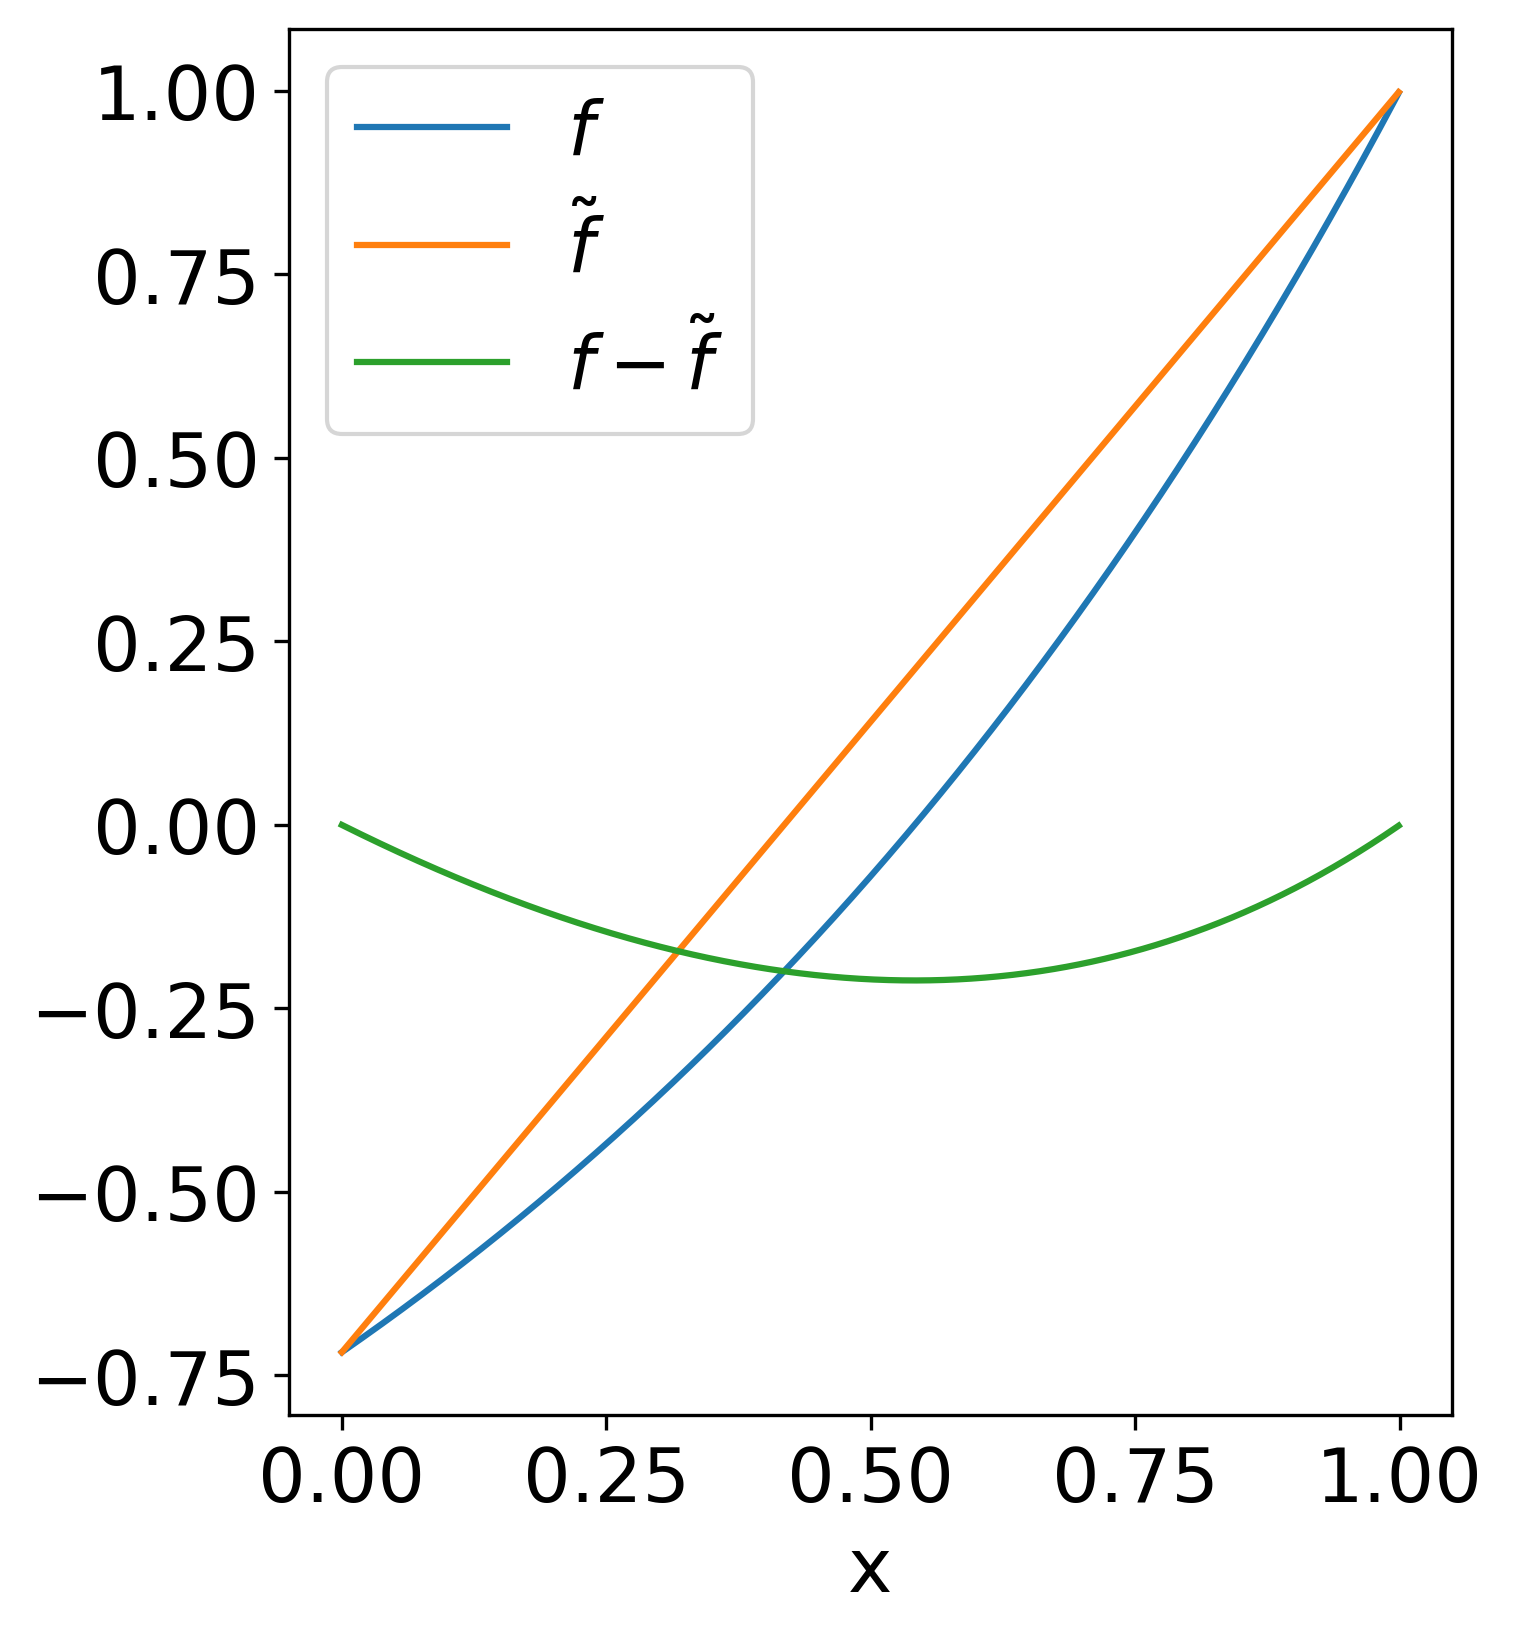
\includegraphics[height=0.8\textheight]{"imgs/control_variate.png"}
            \end{figure}
        \end{column}
        \begin{column}{0.45\textwidth}
            \fontsize{14}{16}\selectfont
            \begin{align*}
                \hspace{0.1cm} & \textcolor{blue!95!black}{\int_{x}^{x+\Delta x} f(s) ds}               \\
                               & = \textcolor{orange!95!black}{\Delta x \frac{f(x) + f(x+\Delta x)}{2}} \\
                               & +E \left[\textcolor{red!90!black}{l B\left( \frac{1}{l}\right)}
                    \textcolor{green!80!black}{(f(S_x) - \tilde{f}(S_x))}\right]
            \end{align*}
        \end{column}
    \end{columns}

\end{frame}


\begin{frame}
    \frametitle{Trapezium Monte Carlo}
    \fontsize{15}{17}\selectfont
    \begin{align}
         & \int_{a}^{b} f(s) ds                                      \\
         & \approx \Delta x \sum_{x}  \frac{f(x) + f(x+\Delta x)}{2} \\
         & + l B\left(\frac{1}{l}\right)
        \left(f(S_x) - f(x) - \frac{S_x - x}{\Delta x}(f(x+\Delta x) - f(x))\right)
    \end{align}
\end{frame}

\begin{frame}
    \frametitle{Trapezium Monte Carlo}
    \vspace{-0.9cm}
    \begin{equation}
        \int_{0}^{1} e^{s} ds, \quad \Delta x = h
    \end{equation}
    \vspace{-1cm}
    \begin{figure}[h]
        \centering
        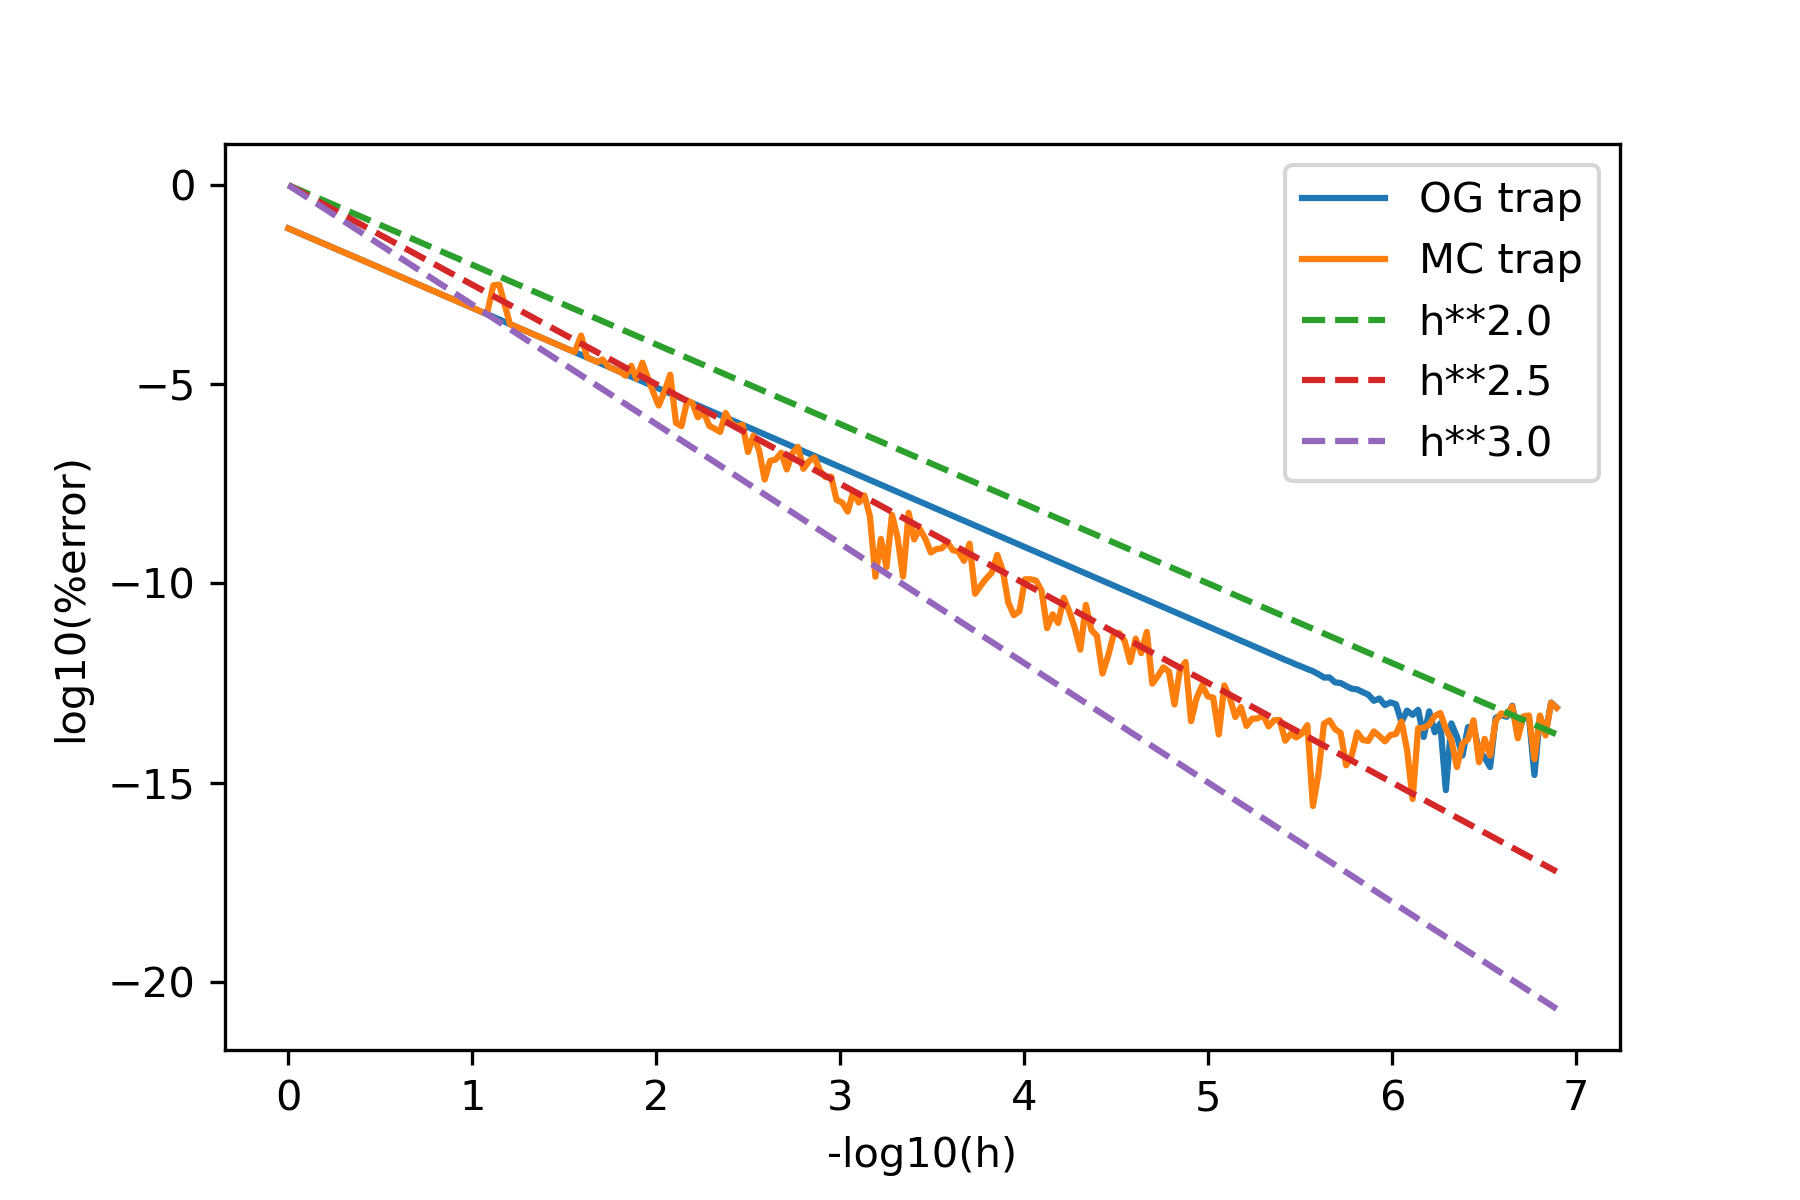
\includegraphics[width=0.8\textwidth]{"imgs/trapMC.png"}
    \end{figure}
\end{frame}

\begin{frame}
    \frametitle{Trapezium Monte Carlo}
    \begin{align}
        \hspace{0.3cm}\|f\|_2 & \leqslant \sqrt{\|f\|_1 \|f\|_{\infty}} \\
        \|f\|_2               & = O(h^{p + \frac{d}{2}})                \\
        \|f\|_{\infty}        & = O(h^{p })                             \\
                              & \downarrow                              \\
        \|f\|_1               & = O\left(h^{p+d}\right) ?
    \end{align}
\end{frame}

% 3 min
\begin{frame}
    \frametitle{RMC voorbeeld}
    \vspace{-2cm}
    \begin{align}
        \action<+->{y'            & =y  }                        \\
        \action<+->{y(t)          & =y(0)+ \int_{0}^{t} y(s)ds } \\
        \action<+->{\text{wil } Y & : E[Y(t)] = y(t)}            \\
        \action<+->{Y(t)          & =y(0)+tY(S) } \label{RRVE}   \\
        \action<.->{S             & \sim \text{Uniform}(0,t)}
    \end{align}
\end{frame}

\begin{frame}
    \frametitle{RMC voorbeeld}
    \vspace{-2cm}
    \begin{align}
        \action<+->{Y(t)    & =y(0)+tY(S) }             \\
        \action<+->{ \infty & \text{ recursie } }       \\
        \action<+->{ Y(t)   & = 1 + B(t)Y(S)}           \\
        \action<.->{ t      & < 1}                      \\
        \action<.->{B(t)    & \sim \text{Bernoulli}(t)}
    \end{align}
    tekening
\end{frame}


% 4 min
\begin{frame}
    \frametitle{RRMC voorbeeld}
\end{frame}

% 6 min
\begin{frame}
    \frametitle{Unbiased non-linearity}
    \begin{itemize}
        \item exponentiele voorbeeld + screenshot paper
        \item VRE
        \item Feynman-Kac formule
        \item Magnus series
    \end{itemize}
\end{frame}

\end{document}